%\documentclass[11pt]{report}



%\begin{document}

\chapter{Technical overview}
\label{ch:tech-overview}
%\addcontentsline{toc}{chapter}{Introduction}

In this chapter, we present the fundamental mathematical and information-theoretic concepts that are utilized throughout the thesis.

\section{Mathematical preliminaries}

In this section, we define and explain the mathematical notation and concepts used throughout the thesis.

First, we use $\gcd(a,b)$ to denote the greatest common divisor between integers $a$ and $b$, with $a,b \in \mathbb{Z}$. We use $\mathbb{Z}_q$ to denote the set of integers $a \mod q$, and $\mathbb{Z}^*_q$ to denote the set of integers $a \in \mathbb{Z}_q$ that are coprime with $q$, i.e., $\gcd(a,q) = 1$. When $q$ is prime, $\mathbb{Z}^*_q$ forms a multiplicative group of order $q-1$ and $\mathbb{Z}_q$ forms a finite field of order $q$. A generator $g$ of a multiplicative group $\mathbb{G}$ is an element in $\mathbb{G}$ such that for all $a \in \mathbb{G}$, there exists an integer $r$ such that $g^r = a$. The discrete logarithm base $g$ of an element $a \in \mathbb{G}$, denoted by $\log_g a$, is the power $r$ of $g$ such that $g^r = a$.

We use $|I|$ to denote the size of a set $I$ and use the notation  $s\leftarrow_{\$}I$ to describe a situation where an element $s$ is drawn uniformly at random from the set $I$. Vectors $\bm{v} = (v_1, \ldots, v_n)$ are denoted in bold. Given a set $J$, $\bm{v}_{|J}$ denotes the subvector of $\bm{v}$ restricted to the indices $i \in J$. For $m \in \mathbb{Z}_q$, $[m]$ is the ordered set ${1, 2, \ldots, m}$, and for $m, n \in \mathbb{Z}_q$ such that $m < n$, $[m, n] = {m, m+1, \ldots, n-1, n}$. For $\bm{x}, \bm{y} \in \mathbb{Z}^n_q$, $r_H(\bm{x}, \bm{y}) = d_H(\bm{x}, \bm{y})/n$ is the relative Hamming distance, where the Hamming distance is given by $d_H(\bm{x}, \bm{y}) = |{i : x_i \neq y_i}|$.

Finally, we use the big-$\mathcal{O}$ notation to denote the fastest-growing term of the number of operations with respect to some security parameter $n$. A negligible function $\mu(n)$ is a function such that $\mu(n) < 1/p(n)$ for some polynomial $p(n)$ and sufficiently large $n$.



%********************************** %First Section  **************************************
\section{Secure multiparty computation}

Secure multiparty computation (SMC) allows multiple parties, denoted as $P_i$ with $i \in {1,\ldots,n}$, to jointly compute a function, $f(x_1,\dots,x_n) = (y_1,\ldots,y_n)$, without revealing their individual inputs, $x_i$, to each other. The only information received by each party $P_i$ is their corresponding output $y_i$ of the function $f()$, which may reveal some information about the parties' inputs depending on the function being computed. This functionality is designed to be equivalent to a scenario where each party $P_i$ sends their input $x_i$ to an independent and trusted third party $P_{\mathsf{TTP}}$, who computes $f(x_1,\ldots,x_n)$ and sends the output $y_i$ to each party.

It is important to note that SMC may not completely hide the inputs of the parties, even with a perfectly secure protocol. This is due to the security guarantees of the ideal scenario, where it is possible for a perfectly legitimate SMC protocol (such as using a trusted third party) to leak all the inputs of the parties. This can happen when one of the parties can use their inputs and outputs to invert the function $f()$. For example, if two parties want to compute the average of their weight, it is straightforward for both parties to use their weight and the average value to compute the other party's weight, as the function is bijective with the adversaries' inputs fixed. In this scenario, SMC does not improve the privacy of the computation.
%Estrutura da introdução:
%
%- Cometar que não sabemos mais do que o output da computação. Dar o exemplo da média de pesos. 2 pessoas sabemos o resultado. 3 já não. Ainda assim, pode revelar alguma coisa a mais. Note that, pratically, we can put together other PET such as Differential Privacy in oder to do this.

The following are some informal descriptions of properties of SMC:

\begin{enumerate}
\item Correctness: If all the parties abide by the protocol, the protocol will evaluate the correct output according to $f()$ and the parties' inputs $x_1, \ldots, x_n$.

\item Passive security: If the adversaries do not deviate from the protocol, they do not learn the inputs of the honest parties. In this thesis, we refer to adversaries who do not deviate from the protocol as semi-honest parties, also known as honest-but-curious adversaries in the literature.

\item Active security: If the adversaries deviate arbitrarily from the protocol (dishonest parties), they do not learn the inputs of the honest parties. In active security, there are two types of protocols that react differently to adversarial behavior. They can be robust against the adversaries, meaning the honest parties will still receive the correct answer, or the honest parties can abort the protocol when there is malicious activity.
\end{enumerate}

Regarding the corruption strategy of the adversaries, they can be of two types: static or adaptive. Static security guarantees that the protocol is secure against an adversary who only corrupts parties before the execution of the protocol. Adaptive security is a more challenging property to attain, as it assumes that the adversary can choose which party to corrupt throughout the protocol. It is also worth noting that there is a fundamental difference between the adversarial structure of encryption methods and SMC methods. In encryption methods, the adversary is considered an external party (usually referred to as Eve) that interferes with the communication between the protocol parties. In the case of SMC methods, the adversaries are a subset of the protocol parties.

Next, we present two common approaches used for SMC protocols: the garbled circuit approach and the secret sharing approach. The garbled circuit approach is generally based on boolean circuits and follows from the techniques developed by Yao \cite{Yao82}. The secret sharing approach is commonly based on arithmetic circuits (although it can also be used with boolean circuits) and follows from the properties of secret sharing \cite{BGW88, CCD88}. It should be noted that throughout this thesis, we will focus on two-party protocols. For this reason, we name these parties Alice and Bob, and follow the convention that Alice plays the role of the protocol's sender and Bob plays the role of the receiver.

\subsection{Garbled circuit approach}

The garbled circuit approach, which is based on Yao's seminal work \cite{Yao82}, proposes a technique to ``encrypt" boolean circuits in such a way that preserves the security requirements of both parties. This ``encrypted'' version is called a garbled circuit and is presented in this section along with the Yao protocol description. This approach is typically best suited for scenarios with higher latency, as it typically requires a fixed number of communication rounds, regardless of the complexity of the function being evaluated. However, for large circuits, high bandwidth is required \cite{PWM+20}.

Before delving into the details of the Yao protocol, it is important to introduce a crucial primitive: oblivious transfer (OT).

\subsubsection{Oblivious transfer}

The study of oblivious transfer (OT) has been active since its first proposal by Rabin in 1981 \cite{Rabin81}. The importance of OT comes from its wide range of applications. In particular, it can be proven that OT is equivalent to the secure two-party computation of general functions \cite{Y86, K88}, meaning that a secure two-party computation can be implemented using OT as its building block. Additionally, this primitive can also be used for secure multiparty computation (SMC) \cite{KOS16}, private information retrieval \cite{Che04}, private set intersection \cite{MEP17}, and privacy-preserving location-based services \cite{BHM+19}.

The OT functionality can be presented in many flavours. In this thesis, when we refer to OT, we mean the $1$-out-of-$2$ OT that is specified in Figure~\ref{fig:OT_functionality}. Consequently, we have that OT must satisfy the following security requirements:

\begin{itemize}
	\item Concealing: Alices knows nothing about Bob's bit choice $b$.
	\item Obliviousness: Bob knows nothing about the message $m_{b\oplus 1}$.
\end{itemize}

OT can be generalized to the case of $k$-out-of-$N$ OT, where Alice owns $N$ messages, and Bob can choose $k$ of them. For $k=1$, this is commonly called private database query (PDQ). Also, we call random OT when both parties' inputs are random.

\begin{figure}[b!]
\centering
\begin{tcolorbox}[enhanced, 
                        frame hidden,
                        ]
                        
    \centerline{$\mathcal{F}_{\textbf{OT}}$ \textbf{functionality}}
            
    \
    
    \begin{itemize}
    		\item \textbf{Input phase:} Alice sends $(m_0, m_1)\in\{0,1\}^l$ (two messages) to $\mathcal{F}_{\textbf{OT}}$ and Bob sends $b\in\{0,1\}$ (bit choice) to $\mathcal{F}_{\textbf{OT}}$.
    		\item \textbf{Output phase:} Alice receives nothing $\bot$ from the functionality and Bob receives $m_b$.
    \end{itemize}
    
\end{tcolorbox} 
    \caption{OT functionality.}
    \label{fig:OT_functionality}
\end{figure}

\subsubsection{Yao protocol}\label{yaoProtocol}

A solution for SMC was first proposed by Yao \cite{Yao82}, where he developed the concept of garbled circuits, which is one of the key elements for secure computation. The Yao's garbled circuit protocol is originally designed for only two parties, but its generalization to multiple parties was later achieved by GMW \cite{Goldreich87} and BMR \cite{BMR90}. Additionally, various implementation optimizations have been developed to improve the performance of the Yao protocol, such as point-and-permute \cite{BMR90}, row reduction \cite{NPS99, Pinkas2009}, FreeXOR \cite{Kolesnikov2005} and half gates \cite{Zahur2015}.

As mentioned before, the main idea of the Yao protocol is to represent the desired function $f()$ as a boolean circuit $C$, i.e. a sequence of logical gates interconnected with wires. After the generation of the circuit $C$, each party will have two distinct roles. Generally speaking, Alice (also known as the garbler) randomly generates keys for each input bit, encrypts each circuit's gate, and sends both elements to Bob (also known as the evaluator). This procedure masks Alice's inputs from Bob. Then, through the oblivious transfer (OT) functionality, Bob receives the keys corresponding to his input bits. This allows to mask Bob's inputs from Alice. Finally, since the evaluator has all the input keys, he can decrypt every gate, and evaluate the circuit. To better understand how the protocol works, let us consider a four-input boolean circuit description of the Millionaires' problem. This problem can be described by the following expression:
\begin{equation}
f(a, b) = 
     \begin{cases} 
      1 & \mathrm{if} \hspace{0.2cm} a>b, \\
      0 & \mathrm{otherwise},
   \end{cases}
\label{eq:MPeq}
\end{equation}   
for $a, b \in \{0,1\}^2$. In summary, it allows two parties to discover who has the largest value without revealing them.

The protocol goes as follows:
\begin{enumerate}
    \item \textit{Circuit generation:} The garbler Alice generates a boolean circuit of function (\ref{eq:MPeq}):
    
    \begin{figure}[h]
        \centering
        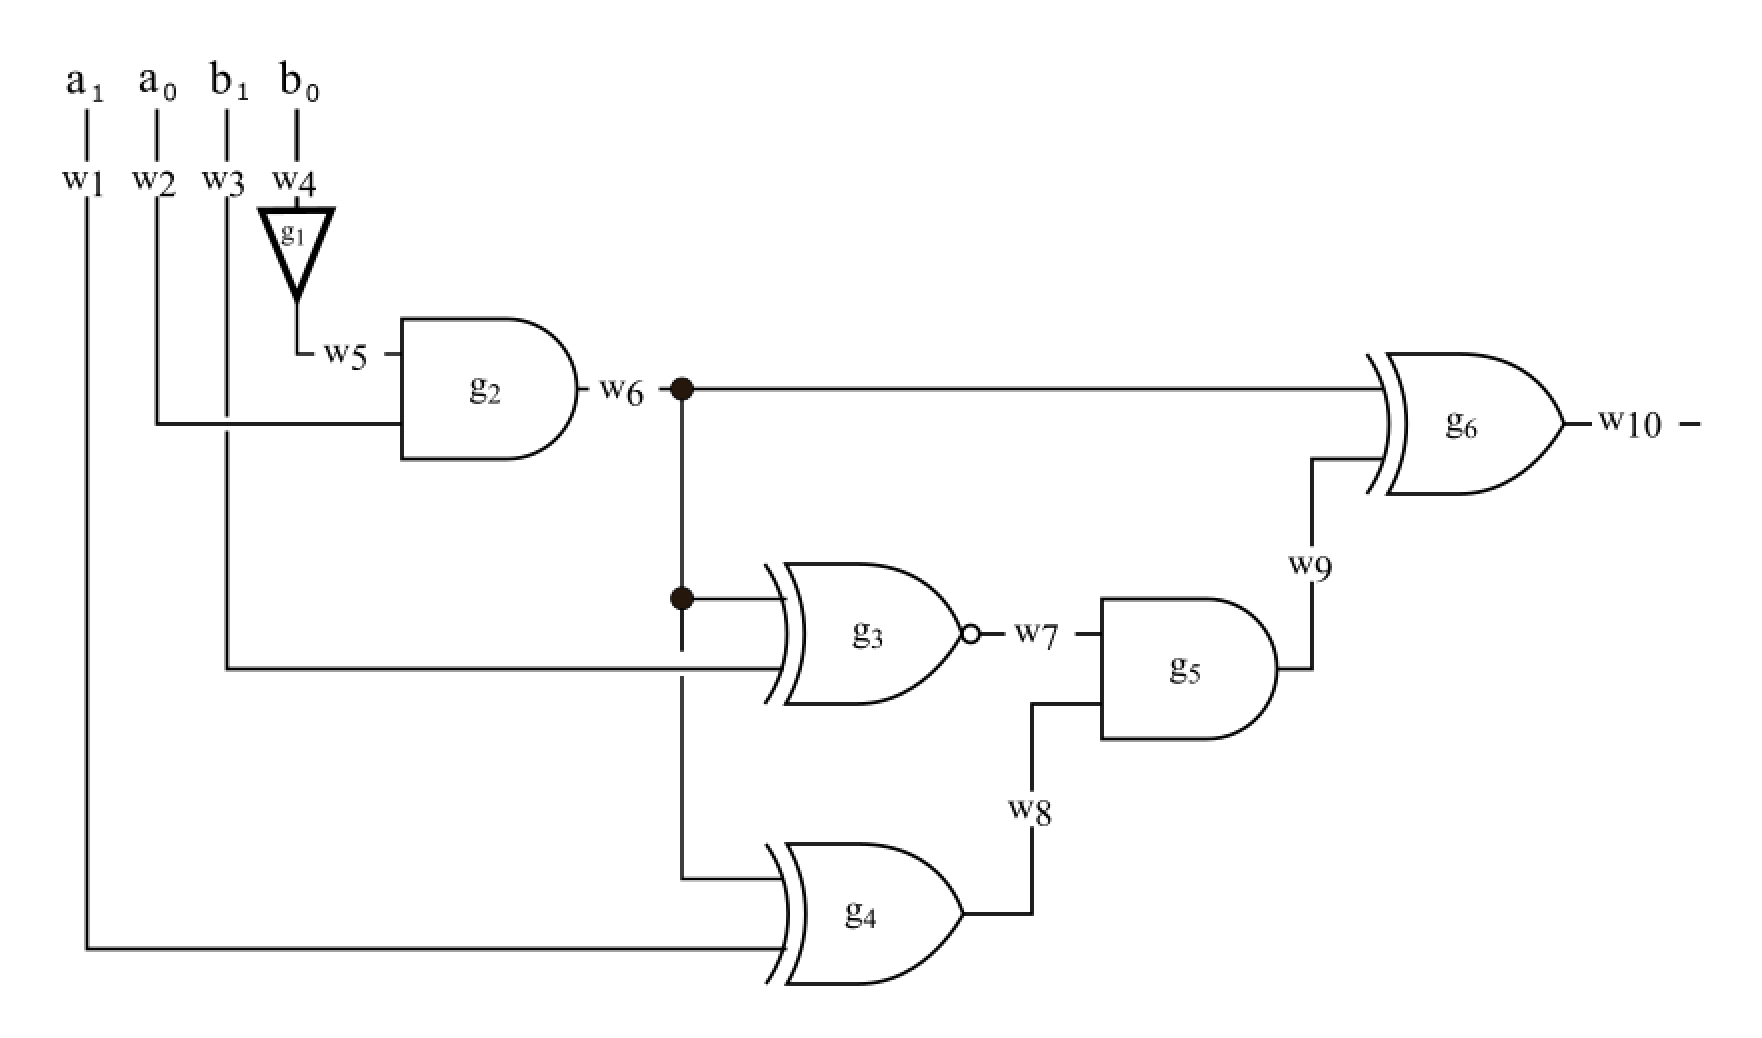
\includegraphics[scale=0.3]{Chapter_TechnicalOverview/booleanCircuit.png}

        \caption{Boolean circuit of the Millionaires' Problem. Optimised circuit according to the construction in \cite{Kolesnikov2009}.}
        \label{fig:boolean}
    \end{figure}
    
    In this case, the circuit contains one NOT gate ($g_1$), two AND gates ($g_2$, and $g_5$), two XOR gate ($g_4$ and $g_6$), one XNOR gate ($g_3$) and four input wires ($w_1$ and $w_2$ belonging to Alice and $w_3$ and $w_4$ to Bob).
    
    \item \textit{Wire encryption:} Alice uses a random number generator to generate two keys $k^0_i$ and $k^1_i$ for each wire $w_i$, $i\in\{1, ..., 10\}$. These keys correspond to the possible values ($0$ or $1$) on the wire. Note that this is done to prevent Bob from knowing the true value of the wires during the evaluation process.
    
    \item \textit{Gate encryption:} For every gate $g_l$ in the circuit with corresponding input wires $w_i$ and $w_j$ and output wire $w_s$, Alice creates the following table:

    \begin{center}
        \begin{tabular}{ |c| } 
        \hline
        $\mathsf{Enc}_{k_i^0}\left(\mathsf{Enc}_{k_j^0}\left(k_s^{g_l(0,0)}\right)\right)$ \\ 
        \hline
        $\mathsf{Enc}_{k_i^0}\left(\mathsf{Enc}_{k_j^1}\left(k_s^{g_l(0,1)}\right)\right)$ \\ 
        \hline
        $\mathsf{Enc}_{k_i^1}\left(\mathsf{Enc}_{k_j^0}\left(k_s^{g_l(1,0)}\right)\right)$ \\ 
        \hline
        $\mathsf{Enc}_{k_i^1}\left(\mathsf{Enc}_{k_j^1}\left(k_s^{g_l(1,1)}\right)\right)$ \\
        \hline
        \end{tabular}
    \end{center}
    
    where $g_l(a,b)$ is the output of gate $g_l$ for inputs $a, b\in \{0, 1\}$. So, we could think of each row as a locked box that requires two keys to be opened. If the two correct keys are used, it outputs the key corresponding to the desired output value given by $g_l$. After encrypting each gate, Alice permutes the rows of the corresponding table, otherwise, it would be easy to know the real value of the input keys. Then, she sends to Bob the garbled tables along with Alice's input keys.
    
    As an example, we can easily see that if we use input keys $k_i^0$ and $k_j^1$ (corresponding to real values $0$ and $1$), we would only be able to decipher the second row of the table, $\mathsf{Enc}_{k_i^0}(\mathsf{Enc}_{k_j^1}(k_s^{g_l(0,1)}))$, and get $k_s^{g_l(0,1)}$.
    
    \item \textit{Oblivious Transfer:} At this stage of the protocol, the evaluator Bob knows the garbled circuit and Alice's input keys but he does not know the keys corresponding to his real inputs. However, since Bob wants to keep his input value private he cannot directly ask for those keys. At this point, the OT functionality enables the evaluator to receive his input keys without compromising neither the evaluator's nor garbler's security. In fact, for every input wire, both parties perform an OT where Alice plays the role of the sender and Bob plays the role of the receiver. 
    
    Let us assume Alice's input keys to be $k_1^0$ and $k_2^1$ (corresponding to the real value  $01$) and Bob's input bits to be $11$. This means that Bob must use the respective input keys ($k_3^1$ and $k_4^1$) in order to correctly evaluate the circuit. So, they will execute two OT protocols where:
    
    \begin{itemize}
        \item Alice inputs: $(k_3^0, k_3^1)$ and $(k_4^0, k_4^1)$;
        \item Bob inputs: $b_1 = 1$ and $b_2 = 1$.
    \end{itemize}
    
    \item \textit{Evaluation:} Once the evaluator has all the necessary elements, he can proceed with the circuit evaluation. In this step, he simply has to decipher the correct rows of the garbled tables sent by Alice with the corresponding keys. Since the rows of the tables are shuffled, the evaluator does not know which row is the correct one. This small issue can be solved by simple techniques (Point-and-Permute or encryption with a certain number of $0$ padded) which, for the sake of brevity, we will not explore here. At the end of the evaluation, the evaluator receives the key that corresponds to the result. Finally, the evaluator sends the resulting key to the garbler and the garbler tells him the final bit.
    
    According to our Millionaires' problem, the evaluation yields the following results for $a = 01$ and $b = 11$: $g_1(k_4^1) = k_5^0$, $g_2(k_5^0, k_2^1) = k_6^0$, $g_3(k_6^0, k_3^1) = k_7^0$, $g_4(k_6^0, k_1^0) = k_8^1$, $g_5(k_7^0, k_8^1) = k_9^0$, $g_6(k_6^0, k_9^0) = k_{10}^0$. Actually, the desired result is $0$.
    
\end{enumerate}


The Yao protocol has its security based on two main building blocks: garbled circuits and oblivious transfer. Although garbled circuits can be generated with symmetric encryption (i.e. using double AES encryption), OT protocols cannot be classically achieved with symmetric cryptography alone \citep{IR89}. Thus, it is crucial to find efficient protocols for a quantum-resistant OT.

%Lindell and Pinkas presented a simulation-based proof that is based on the fact that 
%LP09


%Description
%
%Optimizations
%
%Security
%
%Generalizations of Yao: GMW, BMR

\subsection{Secret sharing approach}

The secret sharing approach, first introduced by BGW \cite{BGW88} and CCD \cite{CCD88}, does not involve encrypting the circuit. Instead, parties use a secret sharing scheme to evaluate the circuit. This approach involves simple operations such as addition and multiplication, but the number of communication rounds needed will depend on the size of the circuit being evaluated. An important primitive for secret sharing based protocols is oblivious linear evaluation (OLE).

\subsubsection{Oblivious linear evaluation}

Oblivious linear evaluation (OLE) can be thought of as a generalization of oblivious transfer (OT) \cite{Rabin81}. It has been shown to be a building block for securely evaluating arithmetic circuits, such as in \cite{AIK11,DKMQ12,GNN17,DGNBNT17}. Specifically, OLE can be used to generate multiplication triples, which are essential for securely computing multiplication gates \cite{DGNBNT17}. OLE also has applications in tasks such as two-party secure computation \cite{IPS09,ADINZ17,BCGI18,HIMV19,CDIKLOV19} and private set intersection \cite{GN19}.


\begin{figure}[h!]
\centering
\begin{tcolorbox}[enhanced, 
                        frame hidden,
                        ]
                        
    \centerline{$\mathcal{F}_{\textbf{OLE}}$ \textbf{functionality}}
            
    \
    
    \begin{itemize}
    		\item \textbf{Input phase:} Alice sends $(a,b)\in\mathbb{Z}_d^2$ (two field elements) to $\mathcal{F}_{\textbf{OLE}}$ and Bob sends $x\in\mathbb{Z}_d$ to $\mathcal{F}_{\textbf{OLE}}$.
    		\item \textbf{Output phase:} Alice receives nothing $\bot$ from the functionality and Bob receives $f(x):= ax + b$.
    \end{itemize}
    
\end{tcolorbox} 
    \caption{OLE functionality.}
    \label{fig:OLE_functionality}
\end{figure}

The OLE functionality specification is presented in Figure~\ref{fig:OLE_functionality}. Similarly, we have that OLE must satisfy the following security requirements:

\begin{itemize}
	\item Concealing: Alices knows nothing about Bob's field element $x$.
	\item Obliviousness: Bob knows nothing about the function $f()$ other than its evaluation at $x$, i.e. $f(x)$.
\end{itemize}

We can also generalize the OLE functionality to a vectorized version. The vector OLE (VOLE) functionality is presented in Figure~\ref{fig:VOLE_functionality}. Note that Bob only inputs one field element $x$ and Alice inputs two vectors. 


\begin{figure}[h!]
\centering
\begin{tcolorbox}[enhanced, 
                        frame hidden,
                        ]
                        
    \centerline{$\mathcal{F}_{\textbf{VOLE}}$ \textbf{functionality}}
            
    \
    
    \begin{itemize}
    		\item \textbf{Input phase:} Alice sends $(\bm{a},\bm{b})\in\mathbb{Z}_d^{2n}$ (two vectors of field elements) to $\mathcal{F}_{\textbf{VOLE}}$ and Bob sends only $x\in\mathbb{Z}_d$ to $\mathcal{F}_{\textbf{VOLE}}$.
    		\item \textbf{Output phase:} Alice receives nothing $\bot$ from the functionality and Bob receives $\bm{f}(x):= \bm{a}x + \bm{b}$.
    \end{itemize}
    
\end{tcolorbox} 
    \caption{VOLE functionality.}
    \label{fig:VOLE_functionality}
\end{figure}


\subsubsection{Basic operations}

To highlight the importance of OLE in secret sharing based SMC protocols, we go through a passively secure protocol \cite{Evans2018}. We consider the two party case (Alice and Bob) where the parties own additive shares of the secret. So, for some secret value $x$, where $x = x_A + x_B$, Alice owns $x_A$ and Bob owns $x_B$. Depending on the circuit, the operations used in the protocol are as follows:

\begin{itemize}
	\item \textbf{Input}. For Alice to secret share her input value $x$, she randomly chooses $x_B$ and sends it to Bob. Alice defines $x_A$ as $x_A = x - x_B$;
	\item \textbf{Addition}. There are two scenarios to consider:
	\begin{itemize}
		\item \textbf{Scalar}. For Alice and Bob to add a scalar to a secret $x$ ($z = a + x$), Alice computes $z_A = a + x_A$ and Bob sets $z_B = x_B$.
		\item \textbf{Shares}. For Alice and Bob to add secrets $x$ and $y$ ($z = x+y$), they individually add their corresponding shares, i.e. $z_A = x_A + y_A$ and $z_B = x_B + y_B$.
	\end{itemize}
	\item \textbf{Multiplication}. There are two scenarios to consider:
		\begin{itemize}
		\item \textbf{Scalar}. For Alice and Bob to multiply a secret $x$ by a scalar $a$ ($z = a \cdot x$), Alice computes $z_A = a \cdot x_A$ and Bob computes $z_B = a \cdot x_B$.
		\item \textbf{Shares}. Observe that, for Alice and Bob to multiply secrets $x$ and $y$ ($z = x\cdot y$), they require some sort of communication to compute cross terms:
		\begin{eqnarray}
		x\cdot y &=& (x_A + x_B)\cdot (y_A + y_B)\\
		&=& x_A\cdot y_A + x_A\cdot y_B + x_B \cdot y_A + x_B\cdot y_B
		\end{eqnarray}
		
		At this point, Alice and Bob can execute two OLEs to secret share the cross terms $x_A\cdot y_B$ and $x_B \cdot y_A$. Indeed, if Alice inputs $(x_A, - s_A)$ and $(y_A, - s'_A)$ for random values $s_A, s'_A$ and Bob inputs $y_B$ and $x_B$, Bob will output $s_B = x_A \cdot y_B - s_A$ and $s'_B = y_A \cdot x_B - s'_A$. Thus, we have that $s_A + s_B = x_A \cdot y_B$ and $s'_A + s'_B = y_A \cdot x_B$. So, Alice share is $z_A = x_A\cdot y_A + s_A + s'_A$ and Bob share is $z_B =  s_B + s'_B + x_B\cdot y_B$.  
	\end{itemize}
	\item \textbf{Output}. For Alice to receive the output value $x$ of some output wire, Bob simply sends $x_B$ to Alice. Alice outputs $x = x_A + x_B$.
\end{itemize}


%********************************** %Second Section  **************************************
\section{Quantum information}

Quantum information theory is a field that studies the implications of using quantum systems as the medium of information. The information carriers in quantum systems are governed by the laws of quantum mechanics, allowing for properties not present in classical methods to be exploited. In this section, we present the basic elements of quantum information that will be used in the quantum protocols presented and their security proofs.

In quantum information theory, a quantum system is described by a Hilbert space $\mathcal{H}_A$. In this thesis, we will consider only finite-dimensional Hilbert spaces, where $\dim \mathcal{H}_A = d < \infty$. The space $\mathcal{H}_A$ can be identified with the complex vector space $\mathbb{C}^d$, as well as its corresponding dual space $\mathcal{H}^{*}_A$. We use the Dirac bra-ket notation to describe the states of a quantum system. A pure state is described by a normalized vector $\ket{\psi}_A \in \mathcal{H}_A$ and its dual vector $\bra{\psi}_A \in \mathcal{H}^{*}_A$. To simplify notation, we may omit specifying the Hilbert space to which a state belongs if it is clear from context. The standard basis of $\mathbb{C}^d$ can be identified with the computational basis of $\mathcal{H}_A$, denoted as $\left\{ \ket{i} \right\}_{i=0}^{d-1}$. The joint system of multiple subsystems $\mathcal{H}_1, \ldots, \mathcal{H}_n$ can be described by their tensor product, denoted as $\mathcal{H}_1 \otimes \ldots \otimes \mathcal{H}_n$. The vectors in this joint system are represented as $\ket{\bm{x}} = \ket{x_1} \otimes \ldots \otimes \ket{x_n}$, where $\bm{x} \in \mathbb{Z}_d^n$.

We can generate quantum pure states, denoted as $\ket{\psi_i}\in \mathcal{H}$, according to a probability distribution ${p_i}$. This situation is described by a density operator, denoted as $\rho = \sum_i p_i \ketbra{\psi_i}$, which is commonly referred to as a mixed state. Density operators are positive semi-definite hermitian operators with unitary trace, that is, $\rho \geq 0$ and $\tr \rho = 1$. The set of hermitian operators, positive semi-definite operators and density operators on a Hilbert space $\mathcal{H}$ are denoted as $\text{Herm}(\mathcal{H})$, $\text{Pos}(\mathcal{H})$ and $\mathcal{P}(\mathcal{H})$ respectively.

A mixed state is considered classical if it is of the form $\rho_{\mathcal{X}} = \sum_{x\in\mathcal{X}} P_X(x)\ketbra{x}$, where $\mathcal{X}$ is a finite set and $P_X$ is a probability distribution over $\mathcal{X}$. The uniform distribution over $\mathcal{X}$ is denoted as $\tau_{\mathcal{X}} = \frac{1}{|\mathcal{X}|}\sum_{x\in\mathcal{X}}\ketbra{x}$, where $|\mathcal{X}|$ is the size of $\mathcal{X}$. The identity operator is denoted by $\mathds{1}$. Additionally, for a bipartite quantum state $\rho_{XB}$, it is said to be a classical-quantum state (cq-state for short) if it is of the form $\rho_{XB} = \sum_{x\in \mathcal{X}} P_X(x) \ketbra{x} \otimes \rho^x_{B}$, where $P_X$ is a probability distribution over the finite set $\mathcal{X}$.

\subsection{Trace distance}

Proving the security of quantum protocols requires a method for distinguishing quantum states. Fortunately, there is a useful metric, known as the trace distance, that measures the distinguishability of two quantum states, $\sigma, \rho \in \mathcal{P}(\mathcal{H})$, by any procedure, regardless of efficiency. The trace distance is defined as \cite{U17}
\begin{equation*}
    \delta(\rho,\sigma):=\frac{1}{2}||\rho-\sigma||_1,
\end{equation*}
where $||\cdot||_1$ is the $1-$Schatten norm in the space of bounded operators acting on a Hilbert space. Its name comes from the fact that we can write it using the trace operator as follows
\begin{equation*}
    ||\rho-\sigma||_1=\Tr\left\{\sqrt{(\rho-\sigma)^\dagger(\rho-\sigma)}\right\}.
\end{equation*}

In this work, we will utilize completely positive trace preserving (CPTP) maps. These maps are defined as preserving the normalization of input states and mapping positive operators to positive operators. As a result, they ensure that density operators are mapped to density operators, making them useful in describing all physically possible operations. They will be a key focus in Chapter~\ref{ch:QOLE}, which deals with the quantum oblivious linear evaluation protocol. However, it is important to note that CPTP maps do not increase the distinguishability between quantum states, as proven in Lemma~\ref{lemma:trace_distance}. In other words, the trace distance between two quantum states remains unchanged after being transformed by a CPTP map.

%{\cv Useful links to support this: \href{https://en.wikipedia.org/wiki/Quantum_operation#Kraus_operators}{wiki} and \href{https://courses.cs.ut.ee/all/MTAT.07.024/2018_fall/uploads/notes.pdf}{Unruh lectures} on pag 16 (def of quantum operations) and Lemma 7}

\begin{lemma}[Lemma 7, \cite{U17}]
The trace distance has the following properties:
\begin{enumerate}
    \item For any CPTP map $\mathcal{E}$ and any $\sigma, \rho \in \mathcal{P}(\mathcal{H})$ we have that
    $$\delta(\mathcal{E}(\sigma), \mathcal{E}(\rho)) \leq \delta(\sigma, \rho).$$
    
    \item Let $\sigma, \sigma' \in \mathcal{P}(\mathcal{H})$ and $\rho \in \mathcal{P}(\mathcal{H}')$. Then,
    $$\delta(\sigma\otimes \rho, \sigma'\otimes \rho) = \delta(\sigma, \sigma').$$
\end{enumerate}
\label{lemma:trace_distance}
\end{lemma}

Although the following lemma is not directly related to the trace distance, it will be used in Chapter~\ref{ch:QOLE} to bound the trace distance between two states.

\begin{lemma}[Corollary 4, \cite{LPTRG13}]
Let $X:=\{x_1, \ldots, x_n\}$ be a list of (not necessarily distinct) values in $[0,1]$ with the average $\mu_X:=\frac{1}{n}\sum_{i=1^n} x_i$. Let $T$ of size $t$ be a random subset of $X$ with the average $\mu_T := \frac{1}{t}\sum_{i\in T} x_i$. Then, for any $\epsilon > 0$, the set $\bar{T} = X\setminus T$ with average $\mu_{\bar{T}} = \frac{1}{n-t}\sum_{i\in K} x_i$ satisfies
$$P\left[ \mu_{\bar{T}} - \mu_T \geq \sqrt{\frac{n(t+1)}{2(n-t)t^2} \log \frac{1}{\epsilon}}  \right] \leq \epsilon.$$
\label{lemma:trace_distance_bound}
\end{lemma}

%%%%%%%%%%%%%%%%%%%%%%%%%%%%%%%%%%%%%%%%%%%%%%%%%%%%%%%%%%%%%%%% HERE

\subsection{Entropy}

Entropy measures are used to quantify the unpredictability of a random variable and the amount of information gained by observing a system. One of the earliest and most widely used classical entropy measures was developed by Shannon in 1948 \cite{S48}. Shannon's entropy measure captures the idea that more predictable events convey less information. The more surprising and unpredictable an event is, the more informative it is. Shannon started by proposing the following function to describe the amount of information an event $A$ has:
$$I(A) = - \log \left( P(A) \right),$$
where $P(A)$ is the probability of event $A$. Shannon's entropy is defined as the average amount of information of all possible events, and, for a discrete random variable X,  is calculated as follows:
$$H(X) = \mathbb{E}\left[ I(X) \right].$$

In the case of a distribution $P(X)$ over the set $\left\{0,1\right\}$ that selects 1 with probability $p$ and 0 with probability $1-p$, the binary entropy is given by the following equation:
$$H(X) = -p \log_2 p - (1-p)\log_2(1-p).$$

Throughout our analysis, we will also frequently use the $d-$ary entropy function, which is a generalization of the standard binary entropy function. However, it should be noted that the $d-$ary entropy does not possess the same operational meaning as the binary entropy measure.

\begin{definition}
For $d\geq 2$, the \textit{d-ary entropy function} $h_d : [0,1]\rightarrow\mathbb{R}$ is given by
$$h_d(x) = x \log_d(d-1) - x \log_d x - (1-x) \log_d (1-x).$$
\label{def:q-ary}
\end{definition}
The $d-$ary entropy is specially useful to bound the size of an important object in coding theory, the Hamming ball. The Hamming ball with radius $\mu$ centered at some point $\bm{r}$ is defined to be the set of vectors $\bm{z}$ at a distance $\mu$ from $\bm{r}$, when the distance is given by the Hamming distance $d_H$. So, we have the following Lemma.

\begin{lemma}[Lemma 5, \cite{V10}]
\label{lemma:hammingBall}
For an integer $d\geq 2$ and $\mu \in [0, 1-\frac{1}{d}]$,
\begin{equation*}
    |\{ \boldsymbol{z}\in \mathbb{Z}_d^{n}: d_H(\boldsymbol{z}, \boldsymbol{r})\leq \mu n \}| \leq d^{h_d(\mu)n}.
\end{equation*}
\end{lemma} 

When proving the security of protocols, it is crucial to understand the worst-case scenario rather than the average behavior. Therefore, the standard binary entropy definitions are not sufficient for securing protocols, and a new measure is needed. This is achieved through the use of min-entropy. Classically, for a finite random variable $X$, where $P(X=x) = p_x$, the min-entropy is defined as:
$$H_{\min}(X) = -\log \max p_x.$$
Operationally, this gives the probability of correctly guessing the element drawn from $X$, when choosing the element $x$ with maximum probability. That is, $P_{\text{guess}} = \max p_x$. This definition can also be extended to cq-states $\rho_{XB}\in\mathcal{P}(\mathcal{H}_A \otimes \mathcal{H}_B)$ as defined in Definition~\ref{def:cqentropy}.

\begin{definition}
\label{def:cqentropy}
Let $\rho_{X B}\in\mathcal{P}(\mathcal{H}_X \otimes \mathcal{H}_{B})$ be a cq-state. The conditional min-entropy is given by
$$H_{\min}(X|B)_{\rho} = -\log P_{\text{guess}}(X|B),$$
where $P_{\text{guess}}(X|B)$ is given by
$$P_{\text{guess}}(X|B) = \max_{\{M_x\}_x} \sum_x p_x \tr\left[M_x \rho_{x}^B\right],$$
where the maximization is taken over all positive operator-valued measures (POVM), i.e. $\left\{ M_x \geq 0 : \sum_x M_x = \mathds{1} \right\}$.
\end{definition}

In Definition~\ref{def:cqentropy}, $P_{\text{guess}}(X|B)$ represents the probability of correctly guessing $x$ given access to system $B$. Additionally, the maximization is taken over the most general type of measurements allowed in quantum mechanics. The following lemma states how min-entropy changes when a fixed bijective function is applied to the classical subsystem of a cq-state. This lemma will be important in the proof of security for the quantum oblivious linear evaluation protocol presented in Chapter~\ref{ch:QOLE}.

\begin{lemma}
Let $\rho_{XB} \in \mathcal{P}(\mathcal{H}_{X}\otimes \mathcal{H}_B)$ be a cq-state and let $f:\mathcal{X} \rightarrow \mathcal{X} $ be a fixed bijective function. Then,
$$H_{\min}(X|B)_{\rho} \leq H_{\min}(f(X)|B)_{\rho}.$$
\label{lemma:bijectivefunction}
\end{lemma}
\begin{proof}
Consider the unitary operator,
$$U = \sum_x \ketbra{f(x)}{x}.$$ 

We check that $U$ is indeed unitary:
\begin{equation*}
U U^{\dagger} = \left(\sum_x \ketbra{f(x)}{x}\right)\left(\sum_{x'} \ketbra{x'}{f(x')}\right) 
= \sum_x \ketbra{f(x)} = I,
\end{equation*}
where in the last step we used the fact that the function $f$ is a bijection. The same holds for $U^{\dagger}U = I$.

Now, observe the following,
\begin{eqnarray*}
H_{\min}(f(X)|B) &=& -\log \max_{\{M_x\}_x} \sum_x p_x \tr\left[M_x \rho_{f(x)}^B\right]\\
&=& -\log \max_{\{M_x\}_x} \sum_x p_x \tr\left[M_x U \rho_{x}^B U^{\dagger}\right]\\
&=& -\log \max_{\{M_x\}_x} \sum_x p_x \tr\left[U^{\dagger} M_x U \rho_{x}^B \right]. 
\end{eqnarray*}

It is important to note that $\left\{ N_x \right\}_x= \left\{U^{\dagger} M_x U\right\}_x$ is also a POVM, as they are all positive semidefinite operators and they sum up to unity. Therefore, we have that $\left\{U^{\dagger} M_x U\right\}_x$ can only decrease the space of possible POVMs, which is why we have:
$$\max_{\{M_x\}_x} \sum_x p_x \tr\left[U^{\dagger} M_x U \rho{x}^B \right] \leq \max_{\{M_x\}_x} \sum_x p_x \tr\left[ M_x \rho{x}^B \right].$$

This means that, 
\begin{equation*}
H_{\min}(f(X)|B) \geq -\log \max_{\{M_x\}_x} \sum_x p_x \tr\left[ M_x \rho_{x}^B \right] = H_{\min}(X|B).
\end{equation*}
\end{proof}

%In the first (quantum) part of the OLE protocol, Alice and Bob generate several random OLE instances based on expression~\eqref{eq:main_relation} and use them as a resource to generate one final OLE. However, by using entanglement, Bob is allowed to have some limited amount of information on Alice's outputs, i.e. on Alice functions $(a_i, b_i)_{i\in [n]}$. To understand the impact this have on the security of the protocol, we use the concept of \textit{min-entropy}. This quantifies the amount of information Bob has about Alice system $A$ given some (possibly quantum) side information $B'$. This measure of uncertainty has an important operational meaning when Alice's system is classical. We have that $H_{\text{min}}(A|B') = - \log P_{\text{guess}}(A|B')$, where $P_{\text{guess}}(A|B')$ is the probability that of Bob guessing Alice's classical state $A$ maximized over any possible measurement on his state $B'$. Throughout this work, $A$ will encode Alice's functions with space denoted by $\mathcal{G}^n$. We present the formal definition of min-entropy below.

The conditional min-entropy can be generalized to the fully quantum case where both systems are quantum (Definition~\ref{def:conditionalquantumminentropy}).

\begin{definition}
\label{def:conditionalquantumminentropy}
Let $\rho_{A B'} \in \mathcal{P}(\mathcal{H}_A \otimes \mathcal{H}_{B'})$ and $\sigma_{B'} \in \mathcal{P}(\mathcal{H}_{B'})$. The \textit{min-entropy} of $\rho_{A B'}$ relative to $\sigma_{B'}$ is given by
$$H_{\text{min}}(A | B')_{\rho|\sigma} = -\log \min\{ \lambda : \lambda \cdot \text{id}_A \otimes \sigma_{B'} \geq \rho_{A B'} \},$$
and 
$$ H_{\text{min}}(A | B')_{\rho} = \sup_{\sigma_{B'}} H_{\text{min}}(A | B')_{\rho|\sigma_{B'}}.$$
\end{definition}

Furthermore, consider the superposition state $\ket{\phi}_{AB'} = \sum_{z\in B}\alpha_z\ket{z} \ket{\psi^z}$ for some set $\mathcal{B}$ and arbitrary coefficients $\alpha_z$. We define $\rho_{AB'} = \ketbra{\phi}_{AB'}$ and the mixture $\tilde{\rho}_{AB'} = \sum_{z\in \mathcal{B}} |\alpha_z|^2 \ketbra{z} \otimes \ketbra{\psi^z}$. The following lemma gives a lower bound on the min-entropy of $\rho_{AB'}$ in terms of the min-entropy of $\tilde{\rho}_{AB'} $.


\begin{lemma}[Lemma 3.1.13, \cite{R06}]
Let $\rho_{AB'}$ and $\tilde{\rho}_{AB'}$ be defined as above. Then,
$$H_{\text{min}}(A | B')_{\rho} \geq H_{\text{min}}(A | B')_{\tilde{\rho}} - \log |\mathcal{B}|.$$
\label{lemma:renner_lower_bound}
\end{lemma}

It is important to understand the changes in min-entropy that occur when a completely positive (CP) map is applied, as this is a crucial aspect of the security proof for the quantum oblivious linear evaluation protocol outlined in Chapter~\ref{ch:QOLE}. It is known that, for a unital CP map $\mathcal{M}$ (i.e. $\mathcal{M}(\mathds{1}) = \mathds{1}$), the conditional min-entropy does not decrease, i.e. $H_{\min}(\mathcal{M}(A)| B) \geq H_{\min}(A| B)$. However, this result alone is insufficient for deriving practical min-entropy bounds. To obtain meaningful bounds for specific operators $\mathcal{M}$, it is necessary to use Lemma~\ref{thm:entaglementSamplingResult}, in conjunction with Lemma~\ref{lemma:quantumrelation} and Lemma~\ref{lemma:classicalquantumrelation}. It is important to note that for clarity, the lemma employs the notation outlined in Chapter~\ref{ch:QOLE}.


\begin{lemma}[Theorem 1, \cite{Dupuis2015}] 
\label{thm:entaglementSamplingResult}
Let $\mathbf{X}$ denote a system with $n$ qudits, and  $\mathcal{M}_{\mathbf{X}\rightarrow \mathbf{F}\mathbf{Y}}$ be a CP map such that $((\mathcal{M}^\dagger \circ \mathcal{M})_{\mathbf{X}}\otimes \text{id}_{\bar{\mathbf{X}}})(\Phi_{\mathbf{X}\bar{\mathbf{X}}}) = \sum_{(\bm{a},\bm{b})\in\mathbb{Z}^{2n}_d} \lambda_{(\bm{a},\bm{b})} \Phi_{(\bm{a},\bm{b})}$. Then, for any partition of $\mathbb{Z}^{2n}_d = \mathfrak{S}_+ \cup \mathfrak{S}_-$ into subsets $\mathfrak{S}_+$ and $\mathfrak{S}_-$, and $\mathcal{M}(\sigma_{\mathbf{X}E}) = \sigma_{\mathbf{F}\mathbf{Y}E}$ we have 
\begin{equation}
    2^{-\text{H}_2(\mathbf{F}\mathbf{Y} | E)_{\sigma_{\mathbf{F}\mathbf{Y}E} | \sigma_{\mathbf{X}E}}} \leq \sum_{(\bm{a},\bm{b})\in\mathfrak{S}_+} \lambda_{(\bm{a},\bm{b})} 2^{-\text{H}_2(\mathbf{X} | E)_{\sigma_{\mathbf{X}E}}} + \left(\max_{(\bm{a},\bm{b})\in\mathfrak{S}_-} \lambda_{(\bm{a},\bm{b})}\right) d^n,
\end{equation}
 where, in general, for a (not necessarily normalized) quantum state $\rho_{AB}\in \mathcal{P}(\mathcal{H}_A\otimes\mathcal{H}_B)$, $\text{H}_2(A|B)$   is the so-called \textit{collision entropy}~\cite{R06}, given as 
\begin{equation*} 
    \text{H}_2(A|B)_{\rho_{AB}}=-\log \left(\Tr{\left(\rho_{B}^{-1/4}\rho_{AB}\rho_B^{-1/4}\right)^2}\right).
\end{equation*}
If we further condition on a general quantum state $\sigma_B\in\mathcal{P}(\mathcal{H}_B)$, we have 
\begin{equation*}
    \text{H}_2(A|B)_{\rho_{AB}|\sigma_B}=-\log \left(\Tr{\left(\sigma_{B}^{-1/4}\rho_{AB}\sigma_B^{-1/4}\right)^2}\right).
\end{equation*}
\end{lemma}

It is interesting to note that when $\mathcal{M}$ is trace preserving, we have,
$$2^{-\text{H}_2(\mathbf{F}\mathbf{Y} | E)_{\sigma_{\mathbf{F}\mathbf{Y}E} | \sigma_{\mathbf{X}E}}} = 2^{-\text{H}_2(\mathbf{F}\mathbf{Y} | E)_{\sigma_{\mathbf{F}\mathbf{Y}E}}}.$$
This follows from the definition of the collision entropy and the fact that $\Tr_{\bm{F} \bm{Y}}\left[ \mathcal{M}(\sigma_{\bm{X} E}) \right] = \sigma_{E}$ \citep{Dupuis2015}. 

%% This definition comes from the fact that a a map M is (\mu-)trace-preserving iff M^\dagger is (\mu-)unital

% Talk a bit about collision entropy. Look at the references here https://arxiv.org/pdf/0807.1338.pdf

Next, we present a chain rule for the collision entropy.

\begin{lemma}[Proposition 8, \cite{MDSFT13}]
For any $\rho_{ABC}\in\mathcal{P}(\mathcal{H}_A\otimes\mathcal{H}_B\otimes\mathcal{H}_C)$, it holds that
$$H_2(A|BC)_{\rho} \geq H_2(AC|B)_{\rho} - \log d_C,$$
where $d_C$ is the rank of $\rho_C$.
\label{lemma:chain_rule}
\end{lemma}

Now, we need a way to relate min-entropy and collision entropy to have useful bounds for min-entropy. This is done through the following two Lemmas.

\begin{lemma}[Lemma 17, \cite{Dupuis2015}]
\label{lemma:quantumrelation}
Let $\rho_{A B'}\in\mathcal{P}(\mathcal{H}_A \otimes \mathcal{H}_{B'})$ and $d_A = \dim\mathcal{H}_A$. Then
$$H_{\min}(A|B')_{\rho} \leq H_2(A|B')_{\rho} \leq 2 H_{\min}(A|B')_{\rho} + \log d_A.$$
\end{lemma}

\begin{lemma}[Lemma 18, \cite{Dupuis2015}]
\label{lemma:classicalquantumrelation}
Let $\rho_{X B'}\in\mathcal{P}(\mathcal{H}_X \otimes \mathcal{H}_{B'})$ be a cq-state. Then
$$H_{\min}(X|B')_{\rho} \leq H_2(X|B')_{\rho} \leq 2 H_{\min}(X|B')_{\rho}.$$
\end{lemma}

Finally, we present a data-processing inequality, which reflects the intuitive idea that the min-entropy of a system $A$, given side information $B$, does not decrease under local physical operations applied to $B$.

\begin{lemma}[Data processing inequality, Theorem 6.19, \cite{T16}]
\label{lemma:data_processing_inequality}
Let $\rho_{A B}\in\mathcal{P}(\mathcal{H}_A \otimes \mathcal{H}_{B})$. Moreover, let $\mathcal{E}$ be a sub-unital CPTP map from system $A$ to $A'$ (i.e. $\mathcal{E}(\mathds{1}_A) \leq \mathds{1}_{A'}$) and $\mathcal{T}$ be a CPTP map from system $B$ to $B'$. Then, the state $\sigma_{A' B'} = \left(\mathcal{E}\otimes \mathcal{T}  \right)\rho_{AB}$ satisfies
$$H_{\min}(A|B)_{\rho}\leq H_{\min}(A'|B')_{\sigma}.$$
\end{lemma}

\subsection{Two-universal functions}

We start by defining a particular set of functions that are usually used to amplify the privacy of the parties' input and output elements. 

\begin{definition}[$\delta-$almost two-universal hash family; two-universal hash family]
A family, $\mathfrak{F}$, of functions, $g$, with domain $D$ and range $R$ is called a $\delta-$almost two-universal hash family if for any two distinct elements $w,w'\in D$ and for $g$ chosen at random from $\mathfrak{F}$, the probability of a \textit{collision} $g(w)=g(w')$ is at most $\delta$. In the special case that $\delta=1/|R|$, where $|R|$ is the size of the range $R$, the family is called \textit{two-universal}. 
\end{definition}

Now, we present a particular two-universal hash family, known as Multi-linear Modular Hashing (MMH), that preserves the structure of the OLE input and output while maintaining its privacy amplification guarantees. This family is based on the modular inner product of vectors \cite{HK97}.
\begin{definition}[Definition 2, \cite{HK97}]
Let $d$ be a prime and let $n$ be an integer $n>0$. Define a family MMH$^*$ (Multi-linear Modular Hashing) of functions from $\mathbb{Z}_d^n$ to $\mathbb{Z}_d$ as follows
$$\text{MMH}^*:= \{ g_x : \mathbb{Z}_d^n\rightarrow \mathbb{Z}_d \, | \, x\in \mathbb{Z}_d^n \},$$
where the functions $g_x$ are defined for any $x = (x_1,\ldots,x_n)$, $m = (m_1,\ldots, m_n) \in \mathbb{Z}_d^n$
$$g_x(m) = x\cdot m \mod d = \sum x_i\, m_i \mod d.$$
\label{def:MMH}
\end{definition}


\begin{theorem}[Theorem 3, \cite{HK97}]
The family MMH$^*$ is two-universal.
\end{theorem}
Halevi and Krawczyk \cite{HK97} actually prove a stronger result, namely that the MMH$^*$ family is \textit{$\Delta-$universal}, which is more general than two-universal. For the sake of simplicity, we only present the simpler version of this theorem here.

The Generalized Leftover Hash Lemma, presented below, is a crucial component in the security proof of Chapter~\ref{ch:QOLE}. It ensures that, after applying a known function $g$ from a two-universal family to a random variable $X$, the resulting random variable $Z = g(X)$ is close to uniform, given some (possibly quantum) side information $E$. This is a high-dimensional version of the Leftover Hash Lemma, which can be easily derived by using Lemma 4 from \cite{TSSR11} with $d_A = d^l$. Note that this is a special version, as Tomamichel et al. in \cite{TSSR11} prove it in the more general case for $\delta-$almost two-universal hash families.

%Next, we state a crucial result that is used to prove the security of the quantum OLE protocol~\footnote{Here we present a multidimensional version of the Generalized Leftover Hash Lemma. This can be easily deduced by using Lemma 4 from Tomamichel et al. work \cite{TSSR11} with $d_A = d$.}. This ensures that, after applying a known function $f$ from a two-universal family to a random variable $X$, the resulting random variable $Z = f(X)$ is close to uniform conditioned on some (possibly quantum) side information $E$. It also describes how close $Z$ is to uniform with respect to the amount of information we have about $X$ conditioned on $E$, i.e. $H_\text{min}(X|E)$.

\begin{lemma}[Generalized Leftover Hash Lemma \cite{TSSR11}]
Let $X$ be a random variable, $E$ a quantum system, and $\mathfrak{F}$ a two-universal family of hash functions from $X$ to $\mathbb{Z}_d^l$. Then, on average over the choices of $g$  from $\mathfrak{F}$, the output $Z := g(X)$ is $\xi$-close to uniform conditioned on $E$, where
\begin{equation}
  \xi = \frac{1}{2}\sqrt{2^{l\log d - H_\text{min}(X|E)}}.  
\end{equation}
 \label{lem:leftover}
\end{lemma}


%********************************** %Third Section  **************************************
\section{Universal composability}

The universal composability (UC) framework, first introduced by Canetti in the classical setting \cite{C20}, was extended to the quantum setting by Unruh, Ben-Or, and Mayers \cite{Unruh04, BenOrMay04} (see also \cite{Unruh10, FS09}). It provides strong composability guarantees by ensuring the security of a protocol is independent of any external execution of the same or other protocols. Both the classical and quantum frameworks use the same ideal-real world comparison structure and consider similar interactions between machines. However, the quantum-UC framework allows for the manipulation of quantum states in addition to classical operations.

Specifically, the quantum-UC security of a protocol $\Pi$ is determined by comparing its execution in a real scenario, where $\Pi$ is executed, to an ideal scenario, where an ideal functionality $\mathcal{F}$ that carries out the same task is executed. The comparison is performed by a special machine called the environment, $\mathcal{Z}$, which supervises the execution of both scenarios and has access to any external information, such as concurrent executions of the same or any other protocol. In the two-party case, the structure of the machines in both scenarios is as follows: in the real scenario, there is the environment $\mathcal{Z}$, the adversary $Adv$, and the two parties, Alice and Bob. In the ideal scenario, there is the environment $\mathcal{Z}$, the simulator $\mathcal{S}$, the two parties Alice and Bob, and the ideal functionality $\mathcal{F}$. Informally, a protocol $\Pi$ is considered quantum-UC secure if the environment $\mathcal{Z}$ cannot distinguish between the execution of $\Pi$ in the real scenario and the execution of the functionality $\mathcal{F}$ in the ideal scenario. Any possible attack of the adversary $Adv$ in the execution of $\Pi$ can be simulated by the simulator $\mathcal{S}$ in the ideal-world execution of $\mathcal{F}$, without any noticeable difference from the point-of-view of the environment $\mathcal{Z}$. As the ideal functionality $\mathcal{F}$ is secure by definition, the real-world adversary is not able to extract any more information than what is allowed by the functionality $\mathcal{F}$.

The formal definition of quantum-UC security can be stated as follows. Let $\Pi$ and $\rho$ represent the real and ideal two-party protocols, respectively. Let $\text{EXEC}_{\Pi^C, Adv, \mathcal{Z}}$ denote the output of the environment $\mathcal{Z}$ at the end of the real execution, where $C$ denotes the corrupted party and $Adv$ denotes the adversary. Similarly, let $\text{EXEC}_{\rho^C, \mathcal{S}, \mathcal{Z}}$ denote the output of the environment $\mathcal{Z}$ at the end of the ideal execution, where $\mathcal{S}$ is the simulator. 

\begin{definition}[Statistical quantum-UC security,  Computational quantum-UC security \cite{Unruh10}]

Let protocols $\pi$ and $\rho$ be given. We say that $\pi$ statistically quantum-UC emulates $\rho$ if and only if for every party, $C$, and for every adversary, $Adv$, there exists a simulator, $\mathcal{S}$, such that for every environment $\mathcal{Z}$, and every $z\in\{0,1\}^*$, $n\in\mathbb{N}$,
\begin{equation*}
    \big|\text{P}[\text{EXEC}_{\Pi^C, Adv, \mathcal{Z}} (n, z) = 1] - \text{P}[\text{EXEC}_{\rho^C, \mathcal{S}, \mathcal{Z}}(n, z) = 1]\big| \leq \mu(n),
\end{equation*}
 where $\mu(n)$ is a negligible function and $n$ is the security parameter. We furthermore require that if $Adv$ is quantum-polynomial-time, so is $\mathcal{S}$. Finally, if we consider quantum-polynomial-time $Adv$ and $\mathcal{Z}$ we have \textit{computational} quantum-UC security.
\label{def:statisticalquc}
\end{definition}



The role of the simulator, $\mathcal{S}$, in the quantum-UC framework is to simulate the execution of the protocol $\Pi$ in such a way that the environment $\mathcal{Z}$ is not able to distinguish between the real execution and the ideal execution. To accomplish this, $\mathcal{S}$ runs a simulated honest party that interacts with the environment, which is acting as the adversary. Additionally, $\mathcal{S}$ controls the dishonest party and their inputs to the ideal functionality $\mathcal{F}$, as well as the external functionality $\mathcal{F}_{\textbf{ext}}$ if used in the real execution.

In order to generate a simulated execution that cannot be distinguished by the environment, $\mathcal{S}$ relies on its ability to extract the inputs provided to the dishonest party by the environment and uses them along with the ideal functionality outputs. Furthermore, $\mathcal{S}$ can reprogram $\mathcal{F}_{\textbf{ext}}$ in the ideal world as needed to produce an indistinguishable simulation of the real world.

In summary, the simulator $\mathcal{S}$ plays a crucial role in the quantum-UC framework by simulating the execution of the real protocol $\Pi$ in the ideal scenario, in order to ensure that the environment $\mathcal{Z}$ is not able to distinguish between the real execution and the ideal execution, thereby providing strong composability guarantees for the protocol $\Pi$.


%\begin{figure}[!htb]
%\minipage{0.32\textwidth}
%\centering
%  \includegraphics[width=4cm]{img/Real_net.png}
%  \caption{Real model.}\label{fig:realmodel}
%\endminipage\hfill
%\minipage{0.32\textwidth}
%\centering
%  \includegraphics[width=4cm]{img/Ideal_net.png}
%  \caption{Ideal model.}\label{fig:idealmodel}
%\endminipage\hfill
%\minipage{0.32\textwidth}%
%\centering
%  \includegraphics[width=4cm]{img/Real_net.png}
%  \caption{Simulator.}\label{fig:simulator}
%\endminipage
%\end{figure}


 
%Regarding the adversarial model, we consider both \textit{semi-honest} and \textit{dishonest} adversaries. Semi-honest adversaries (also called honest-but-curious or passive adversaries) do not deviate from the protocol and only try to passively gain extra information by looking at the exchanged messages. Dishonest adversaries may deviate arbitrarily from the protocol. We also adopt the static corruption adversarial model where the corruption of each party is done just before the execution of the protocol.

\begin{figure}[]
\centering
\begin{tcolorbox}[enhanced, 
                        frame hidden,
                        ]
                        
    \centerline{$\mathcal{F}_{\textbf{COM}}$ \textbf{functionality}}
            
    \
    
    \begin{itemize}
        \item \textbf{Commitment phase}. Upon receiving $( \texttt{commit}, M)$ from Bob, the functionality sends $\texttt{commit}$ to Alice. 
        \item \textbf{Opening phase}. Upon receiving $\texttt{open}$ from Bob, the functionality sends $(\texttt{open}, M)$ to Alice. 
    \end{itemize}
    
\end{tcolorbox} 
    \caption{Commitment functionality.}
    \label{fig:func_com}
\end{figure}


\subsubsection{Ideal functionalities}\label{functinalities}

Whenever a protocol $\Pi$ utilizes an external functionality $\mathcal{F}_{\textbf{ext}}$, we say that $\Pi$ is in the $\mathcal{F}_{\textbf{ext}}-$hybrid model. The quantum OLE protocol $\Pi_{\textbf{QOLE}}$ presented in Chapter~\ref{ch:QOLE} employs the ideal commitment functionality, $\mathcal{F}_{\textbf{COM}}$, defined in Figure~\ref{fig:func_com}. Note that the protocol makes multiple calls to $\mathcal{F}_{\textbf{COM}}$ and only opens a subset of the committed elements. To specify different instance calls, we use an index element $i$. In the commitment phase, Bob sends $(\texttt{commit}, i, M)$ to the functionality, which in turn sends $(\texttt{commit}, i)$ to Alice. In the opening phase, Bob sends $(\texttt{open}, i)$, and the functionality sends $(\texttt{open}, i, M)$ to Alice.

The $\mathcal{F}_{\textbf{COM}}$ functionality can be replaced by the commitment protocol $\Pi_{\textbf{COM}}$ presented in \cite{CF01}, which is computationally UC-secure in the Common Reference String (CRS) model. As analyzed in \cite{CBGLM21} (Theorem 3.), the protocol $\Pi_{\textbf{COM}}$ computationally quantum-UC realizes $\mathcal{F}_{\textbf{COM}}$ in the CRS model. Therefore, since $\Pi_{\textbf{QOLE}}$ is proved to be quantum-UC secure, the resulting protocol $\Pi_{\textbf{QOLE}}^{\Pi_{\textbf{COM}}}$ is quantum-UC secure by the composition theorem \citep{Unruh10}.


%\begin{figure}[!h]
%\centering
%\framebox[\linewidth][l]{%
%    \parbox{0.95\linewidth}{%
%    \begin{center}
%        \textbf{$\mathcal{F}_{\textbf{COM}}$ functionality}
%    \end{center}
%    
%    \textbf{Committer message:} $M$
%    
%    \begin{itemize}
%        \item \textit{Commitment phase}. Upon receiving $( \texttt{commit}, M)$ from Bob, the functionality sends $\texttt{commit}$ to Alice. 
%        \item \textit{Opening phase}. Upon receiving $\texttt{open}$ from Bob, the functionality sends $(\texttt{open}, M)$ to Alice. 
%    \end{itemize}
%    }%
%}
%\caption{Commitment functionality definition.}
%\label{fig:func_com}
%\end{figure}


\section{Conclusion}

Throughout this chapter, we introduce the essential concepts that underpin the rest of the thesis. The chapter is divided into four main sections. First, we provide a succinct overview of the mathematical notation. Next, we give an informal description of secure multiparty computation. Finally, we introduce the basic formalism of quantum information and the universal composability framework in the quantum setting.


%\bibliography{bibforthesis}
%\bibliographystyle{unsrt}
%\end{document}
